\documentclass[11pt]{article}

% --- packages (all standard; compiles on arXiv / Overleaf) ------------------
\usepackage[margin=1in]{geometry}
\usepackage{amsmath,amssymb}
\usepackage{graphicx}
\usepackage{booktabs}
\usepackage{microtype}
\usepackage[numbers,sort&compress]{natbib}
\usepackage[colorlinks=true,allcolors=blue]{hyperref}
\usepackage{authblk}

\graphicspath{{./}}
\newcommand{\dpcc}{\ensuremath{\Delta\text{PCC-top50}}}

\title{\textbf{Adaptivity Without Reward: A Negative Result for\\
Closed-Loop Region Acquisition in Spatial Transcriptomics}}

\author[]{Ayush Deo}
\author[]{Vrundan Sojitra}
\author[]{Sanjana Pathi}
\affil[]{University of Southern California}
\date{}

\begin{document}
\maketitle

\begin{abstract}
Spatial transcriptomics (ST) is expensive, and region-based platforms force a budget: an operator
must decide \emph{which} regions of a tissue to profile, then reconstruct the rest. A natural and
increasingly fashionable idea is to make this decision \emph{adaptive}---a closed-loop ``agent'' that
conditions each next region on the expression measured so far. We test this idea directly. We build a
reproducible acquisition simulator on HEST-1k~\citep{jaume2024hest}, a strong frozen pathology
encoder~\citep{chen2024uni}, and three imputers spanning a stationary $k$-nearest-neighbor
interpolator, a learned non-stationary regression-kriging model, and an STFlow-inspired imputer with a
nonlinear backbone and iterative spatial message passing~\citep{huang2025stflow}. Against principled
non-adaptive placement baselines from Gaussian-process sensor-placement theory~\citep{krause2008near},
we find that \emph{across seven slides and all three imputers, no closed-loop policy significantly
beats the best non-adaptive placement at any budget}: every $\mathrm{ours}-\mathrm{best\text{-}non\text{-}adaptive}$
95\% confidence interval lies at or below zero. Apparent single-slide wins under the strong imputer
disappear under cross-slide bootstrap. We further show \emph{why}: conditioning the policy on measured
expression yields a real, robust improvement over an image-only variant---but only under the
data-dependent (STFlow-class) imputer, exactly the precondition sensor-placement theory names, and even
then only enough to \emph{tie}, never beat, one-shot placement. The practical message is concrete: for
budget-constrained ST reconstruction, invest in placement and imputation, not in adaptivity.
\end{abstract}

\section{Introduction}

\paragraph{Budget-constrained region selection is a real operational problem in ST.}
Whole-transcriptome spatial assays remain costly and throughput-limited, and an important class of
platforms---region-of-interest systems such as GeoMx DSP~\citep{merritt2020geomx}---profile only a
small, operator-chosen subset of a tissue's regions. The chosen regions are measured; the rest of the
slide is left unprofiled and, if needed, must be \emph{reconstructed}, typically by predicting
expression from co-registered H\&E morphology, a task with an established but bounded accuracy
ceiling~\citep{jaume2024hest,xie2023bleep}. Region selection is therefore not a modeling convenience
but a genuine decision with a genuine cost, and how well it is made directly determines how much of the
transcriptome one recovers per dollar.

\paragraph{The intuitive fix is to make selection adaptive---and that intuition is what we test.}
Because each measurement reveals real expression, it is natural to expect that a \emph{sequential,
closed-loop} policy---one that conditions the next region on the values measured so far---should
outperform a \emph{one-shot} rule that commits to all regions up front. This is the ``active feature
acquisition'' intuition~\citep{yin2020afa}, and it is the implicit promise of recent ``agentic'' framings
of experimental design. The deployed incumbents in ST, however, are all non-adaptive: static gene-panel
selectors~\citep{covert2023persist,reconst2026} and one-shot, diversity-based ROI
rankers~\citep{spatialfinder2026}. If adaptivity helps, there is an obvious gap to fill; if it does not,
the field should know before building the machinery.

\paragraph{We built the agent, and it does not win.}
We construct a wet-lab-free acquisition simulator on HEST-1k, hold the image encoder and imputer frozen
and identical across all policies for fairness, and compare a closed-loop greedy policy (and a clean
adaptive max-uncertainty policy) against the non-adaptive placement rules that Gaussian-process
sensor-placement theory identifies as near-optimal for reconstructing a spatial field: variance-greedy
and mutual-information-greedy placement, which are submodular and hence $(1-1/e)$-optimal~\citep{krause2008near}.
Across a budget sweep from 0.5\% to 20\% of regions, on seven slides spanning four tissues, and under
three imputers of increasing strength---a stationary kNN, a learned regression-kriging, and an
STFlow-inspired graph imputer~\citep{huang2025stflow}---the closed loop never significantly beats the
best non-adaptive placement. Single-slide point estimates occasionally favored the closed loop by a few
thousandths of a PCC point; a cross-slide bootstrap shows these to be noise.

\paragraph{Contributions.}
(i) A clean formalization of closed-loop region acquisition for ST reconstruction and an open,
reproducible benchmark that pairs it with the correct non-adaptive baselines. (ii) A cross-slide
negative result: adaptivity provides no significant gain at any budget under any of three imputers, up
to an STFlow-class model. (iii) A confirmed \emph{mechanism}: the closed loop extracts real signal from
measured expression only when the imputer's posterior is data-dependent---the precondition predicted
by~\citet{krause2008near}---and even then insufficiently to overtake one-shot placement. (iv) A precise,
actionable takeaway and a falsifiable condition under which adaptivity \emph{would} pay. The value of the
result is redirection: it closes a tempting but unproductive direction with evidence and theory rather
than assertion.

\section{Experimental setup (brief)}
\label{sec:setup}

Full methods are in Section~\ref{sec:methods}; the minimum needed to read the results follows. A
\textbf{slide} is partitioned into 112\,$\mu$m square \textbf{regions}, each equal to one 224\,px UNI2-h
patch at 20$\times$~\citep{chen2024uni}; per-region inputs are frozen UNI2-h embeddings and (as ground
truth) log1p pooled expression. The \textbf{target} is Pearson correlation (PCC) over the top-50 highly
variable genes, scored on the \textbf{unprofiled} regions only, following the HEST-Benchmark
protocol~\citep{jaume2024hest}. A \textbf{policy} reveals regions sequentially under a budget (a fraction
of all regions); a frozen, shared \textbf{imputer} then reconstructs the unprofiled regions. We evaluate
three imputers---\textbf{kNN} (stationary), \textbf{kriging} (learned, linear, non-stationary), and
\textbf{graphflow} (STFlow-inspired)---and nine policies, including the non-adaptive placement rules
variance-greedy and MI-greedy~\citep{krause2008near}, a one-shot diversity ranker
(SpatialFinder-style)~\citep{spatialfinder2026}, our closed-loop greedy, a clean adaptive
max-uncertainty policy, and an image-only ablation of our policy. Experiments span seven slides
(prostate $\times 1$, kidney $\times 2$, lung $\times 2$, colon $\times 2$). We \textbf{pre-registered}
the decision rule before the multi-slide run: a closed-loop \emph{win} requires the paired margin
$\mathrm{ours}-\mathrm{best\text{-}non\text{-}adaptive}$ to be positive with a 95\% bootstrap CI
excluding zero at at least one budget; otherwise the negative result stands. ``Best non-adaptive'' is
taken per slide as the maximum over all non-adaptive baselines---the hardest, fairest opponent.

\section{Results}

\paragraph{3.1 The closed loop does not beat non-adaptive placement---on any imputer, at any budget.}
Table~\ref{tab:margins} reports the pre-registered contrast, the paired margin
$\mathrm{ours}-\mathrm{best\text{-}non\text{-}adaptive}$ in PCC-top50, as mean [95\% bootstrap CI] over
the seven slides. Under the stationary kNN and the linear kriging imputer, the margin is negative and
its CI excludes zero at essentially every budget---the closed loop is \emph{significantly worse} than
simply placing regions well. Under the STFlow-class graphflow imputer the margin shrinks toward zero as
budget grows, reaching $-0.005\,[-0.017,+0.003]$ at 10\% and $-0.004\,[-0.009,+0.001]$ at 20\%---a
statistical \emph{tie}, with the point estimate still negative. \textbf{No budget, under any imputer,
yields a positive margin with a CI excluding zero.} The pre-registered win set is empty. The same
graphflow configuration had shown apparent wins of $+0.002$ to $+0.006$ on the single prostate slide
(the budget-sweep gate passed at 5/10/20\%); those margins are smaller than the random baseline's own
seed-to-seed standard deviation, and the seven-slide bootstrap confirms they were noise
(Figure~\ref{fig:gap}a).

\begin{table}[t]
\centering
\caption{Paired margin $\mathrm{ours}-\mathrm{best\text{-}non\text{-}adaptive}$ (PCC-top50, mean [95\% CI],
7 slides). Negative favors non-adaptive placement. No cell is positive with a CI excluding zero.}
\label{tab:margins}
\begin{tabular}{lccc}
\toprule
Budget & kNN & kriging & graphflow (STFlow-class) \\
\midrule
0.5\% & $-0.065\,[-0.163,-0.002]$ & $-0.107\,[-0.199,-0.017]$ & $-0.141\,[-0.231,-0.059]$ \\
1\%   & $-0.097\,[-0.150,-0.055]$ & $-0.158\,[-0.284,-0.052]$ & $-0.109\,[-0.147,-0.069]$ \\
2\%   & $-0.087\,[-0.126,-0.048]$ & $-0.195\,[-0.331,-0.069]$ & $-0.055\,[-0.086,-0.027]$ \\
5\%   & $-0.099\,[-0.152,-0.054]$ & $-0.204\,[-0.370,-0.056]$ & $-0.021\,[-0.043,-0.005]$ \\
10\%  & $-0.113\,[-0.158,-0.071]$ & $-0.116\,[-0.232,-0.037]$ & $-0.005\,[-0.017,+0.003]$ \\
20\%  & $-0.133\,[-0.169,-0.094]$ & $-0.134\,[-0.157,-0.110]$ & $-0.004\,[-0.009,+0.001]$ \\
\bottomrule
\end{tabular}
\end{table}

\begin{figure}[t]
\centering
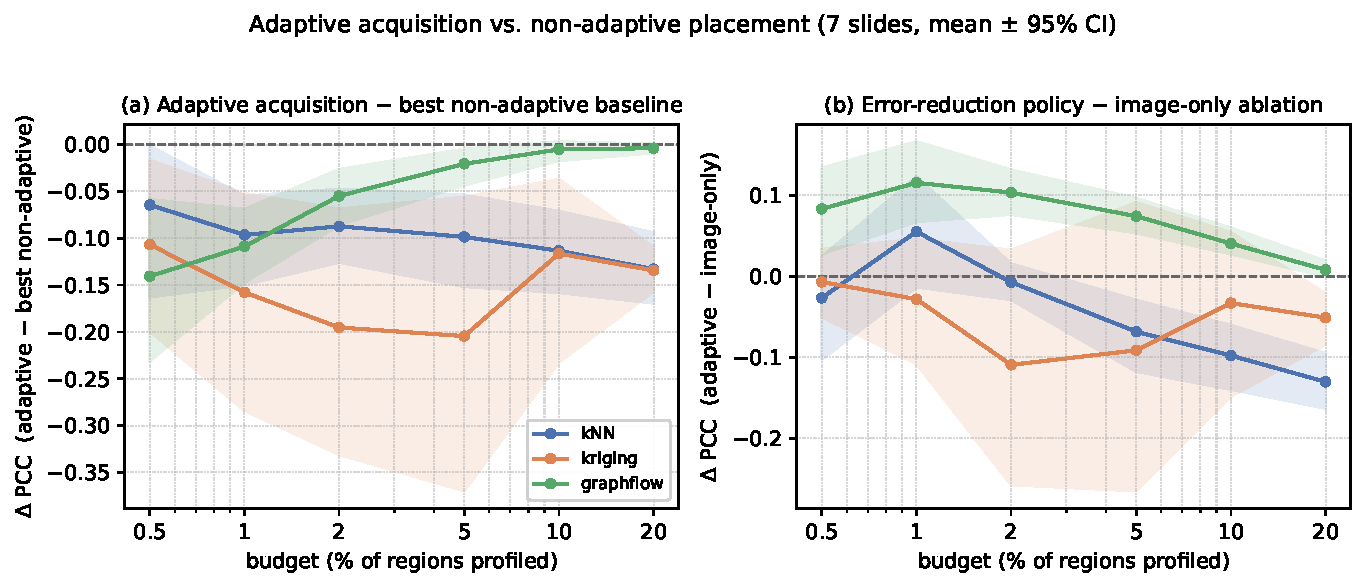
\includegraphics[width=\textwidth]{figure1_adaptivity_gap.pdf}
\caption{\textbf{(a)} The adaptivity gap $\mathrm{ours}-\mathrm{best\text{-}non\text{-}adaptive}$
(PCC-top50) vs budget, per imputer, mean $\pm$ 95\% bootstrap CI over 7 slides. Every band lies at or
below the dashed zero line; the STFlow-class imputer (green) rises toward parity \emph{from below} as
budget grows but never crosses zero. \textbf{(b)} The mechanism contrast
$\mathrm{ours}-\mathrm{image\text{-}only\ ablation}$: conditioning the policy on measured expression is
significantly positive only under the data-dependent graphflow imputer (green), and null-to-negative
under the stationary/linear imputers.}
\label{fig:gap}
\end{figure}

\paragraph{3.2 One-shot placement is near-optimal for reconstruction.}
The reason the closed loop cannot win is that its non-adaptive opponents are already excellent. Averaged
over the seven slides under the strong graphflow imputer, mutual-information-greedy and k-means placement
reach PCC-top50 of 0.588 and 0.587 at 2\% budget and 0.682 and 0.679 at 20\%, essentially matching the
per-slide best non-adaptive value (0.595 and 0.684); the closed-loop policy reaches 0.540 and 0.681. The
one-shot diversity ranker~\citep{spatialfinder2026} is the lone weak non-adaptive method (near-zero PCC
at low budget), consistent with it optimizing for outlier coverage rather than reconstruction. We stress
that our SpatialFinder-style policy is a \emph{reimplementation} of the published diversity-ranking idea,
not the authors' system, and its near-zero low-budget PCC likely reflects an imperfect port rather than
the method's intrinsic ceiling; crucially, because we take the opponent per slide as the \emph{best}
non-adaptive method, this policy is never the ``best non-adaptive'' baseline at any budget, so the verdict
does not depend on the fidelity of our port. The result matches the theoretical expectation: for
reconstructing a spatial field, mutual-information placement is submodular and near-optimal, and---for a
fixed-kernel posterior---is computable offline~\citep{krause2008near}.

\paragraph{3.3 Mechanism: measured expression helps the policy only when the imputer is data-dependent---and not enough.}
The negative result is not because measured values are uninformative; it is because placement already
captures what matters. We isolate the marginal value of \emph{conditioning the policy on measured
expression} with the contrast $\mathrm{ours}-\mathrm{image\text{-}only\ ablation}$ (same policy, same
imputer, with the measured signal switched off in the selection rule). Under the stationary kNN and
linear kriging imputers this contrast is null or negative---measuring gives the policy nothing to act on.
Under the STFlow-class graphflow imputer it is \textbf{significantly positive}: $+0.116\,[+0.068,+0.166]$
at 1\% and $+0.103\,[+0.076,+0.132]$ at 2\% budget, positive on \textbf{7 of 7 slides}, shrinking to
$+0.008\,[-0.000,+0.019]$ at 20\% as the task saturates (Figure~\ref{fig:gap}b). This is precisely the
behavior sensor-placement theory predicts: a closed loop can exploit measured values only when the
imputer's posterior depends on them, i.e.\ when the imputer is non-stationary~\citep{krause2008near}. The
STFlow-class imputer is the first in our ladder to make that dependence strong enough to register---yet
the resulting boost only lets the closed loop \emph{catch} one-shot placement at high budget, never
overtake it, while it still \emph{loses} at the low budgets ($\le 2\%$) where the acquisition decision
matters most.

\paragraph{3.4 The adaptivity gap closes from below and never crosses zero.}
Reading Table~\ref{tab:margins} across imputers traces a clean trend: the margin
$\mathrm{ours}-\mathrm{best\text{-}non\text{-}adaptive}$ at 20\% budget moves from $-0.133$ (kNN) to
$-0.134$ (kriging) to $-0.004$ (graphflow) as the imputer becomes more strongly data-dependent.
Adaptivity's value thus grows monotonically with imputer data-dependence---qualitatively
as~\citet{krause2008near} implies---but it approaches parity \emph{from below} and does not become a
positive, significant gain even at the STFlow-class limit. The strong imputer buys a tie, not a win.

\paragraph{3.5 Robustness and scope of the claim.}
Three points bound the result honestly. (i) The margins are paired within slide and aggregated across
seven slides from four tissues; the deterministic policies carry no within-slide error bars, so all
uncertainty is the cross-slide bootstrap, and the sign split (e.g.\ 0/7 positive for
$\mathrm{ours}-\mathrm{best\text{-}non\text{-}adaptive}$ under graphflow at 0.5--5\%) corroborates the CIs.
(ii) The single strong imputer is STFlow-\emph{inspired}---it carries STFlow's inductive biases (nonlinear
backbone, spatial graph, neighbor-conditioning, iterative refinement) at a scale runnable inside the
acquisition loop, not a 1:1 reproduction; a full flow-matching graph transformer trained cross-slide
could in principle behave differently, though our trend gives no indication it would cross zero. (iii)
Cross-slide absolute PCC is lower than on the single prostate slide (e.g.\ graphflow best-non-adaptive at
20\% is 0.684 across slides vs 0.878 on prostate alone), because kidney, lung, and colon are harder; this
makes the pooled evidence more conservative, not less.

\section{Why adaptivity provides no gain}
\label{sec:why}

\paragraph{The stationary case is a theorem, not an accident.}
For a Gaussian process with a fixed, known kernel, the posterior variance at any location depends only
on \emph{which} locations have been observed, not on the \emph{values} observed there~\citep{krause2008near}.
Consequently the variance-minimizing (or mutual-information-maximizing) set of measurement locations can
be computed entirely offline, and observing the measured values cannot improve the plan: the adaptive and
non-adaptive optima coincide, and the adaptivity gap is exactly zero. Our kNN imputer is precisely this
fixed-kernel regime---its neighbour structure, and hence its predictive uncertainty, is a function of the
region features alone. Theory therefore predicts that no closed loop can help under kNN, and
Table~\ref{tab:margins} confirms it: the margin is not merely $\le 0$ but significantly negative, and it
\emph{worsens} with budget ($-0.065$ at 0.5\% to $-0.133$ at 20\%) as the closed-loop policy's
over-clustering compounds. The same theory supplies the opponents we should fear: mutual-information
placement is submodular, so greedy selection is $(1-1/e)$-optimal and provably strong~\citep{krause2008near}.

\paragraph{The non-stationary case admits a gap in principle---but it stays closed here.}
When the imputer's posterior \emph{does} depend on the measured values (a non-stationary or learned
model), the adaptive and non-adaptive optima can diverge, and a closed loop \emph{can} in principle help.
Our kriging and graphflow imputers are constructed to be non-stationary, and the mechanism contrast
confirms the dependence is real and, for graphflow, strong: conditioning the policy on measured
expression improves it by up to $+0.116$ PCC on 7/7 slides (Section~3.3, Figure~\ref{fig:gap}b). Yet the
realized adaptivity gap never becomes positive (Figure~\ref{fig:gap}a). The reason is quantitative: the
value of \emph{adaptively reallocating} a measurement budget is small relative to the value of \emph{good
coverage}, which principled one-shot placement already secures. A measured value tells the policy
something about where residual error concentrates, but that signal is dominated by what the
image-and-space prior already reveals---the same prior the non-adaptive rule uses to place regions
near-optimally. Non-stationarity of the imputer is thus a \emph{necessary} condition for a gap (met by
graphflow, absent in kNN) but not a \emph{sufficient} one.

\section{Discussion}

\paragraph{When would adaptivity pay?}
Our result localizes the condition rather than merely denying the benefit. A closed loop should be
expected to help when the imputer's predictive posterior is not just data-dependent but \emph{sharply}
so---where a single measurement strongly and non-locally reconcentrates where the model expects error.
Candidate regimes: strongly heteroscedastic or generative imputers whose uncertainty collapses unevenly
after each observation; extreme low-budget settings with strong, structured priors; and batch/multi-round
designs where a first coarse pass reshapes a second. These are falsifiable: each predicts a positive
$\mathrm{ours}-\mathrm{best\text{-}non\text{-}adaptive}$ margin with a CI excluding zero, which our
protocol would detect. Our trend---the gap approaching zero \emph{from below} as imputer data-dependence
increases---offers no evidence that any of these crosses zero, but it does not rule them out, and it
names exactly what a future method must demonstrate.

\paragraph{Practical takeaway.}
For budget-constrained ST reconstruction today, the accuracy lever is not adaptivity. It is the encoder
and imputer (which set the achievable PCC) and principled one-shot placement (which nearly saturates the
acquisition decision). Mutual-information or coverage placement, computed offline, is the recommendation;
a closed-loop acquisition agent adds engineering and compute for no measurable reconstruction return.

\paragraph{Limitations.}
(i) Our strong imputer is STFlow-\emph{inspired}, carrying STFlow's inductive biases at a scale runnable
in-loop, not a 1:1 flow-matching reproduction. (ii) We use HEST Visium HD slides as a stand-in for the
ROI platforms (e.g.\ GeoMx) whose acquisition economics motivate the problem; the region abstraction
transfers but the exact cost model does not. (iii) Evidence is seven slides across four tissues with a
top-50-HVG primary metric; broader tissue and whole-transcriptome sweeps would tighten the CIs further.

\section{Related work}

\paragraph{Predicting expression from morphology, and its ceiling.}
A large body of work maps H\&E to spatial expression---contrastive retrieval~\citep{xie2023bleep},
flow-matching over spatial neighbourhoods~\citep{huang2025stflow}, diffusion models~\citep{zhu2025stem},
and autoregressive gene-structure models~\citep{genar2025}---benchmarked on HEST-1k~\citep{jaume2024hest},
whose scaling analysis shows accuracy rising with encoder capacity. A consistent finding is that
morphology predicts a marker subset well and most genes weakly; this bounded ceiling is the backdrop
against which \emph{any} acquisition method operates, and it is why we hold the encoder fixed and study
selection in isolation.

\paragraph{Selecting what to measure---non-adaptively.}
Existing ST selection methods are one-shot. Gene-panel selectors choose a static informative gene
subset~\citep{covert2023persist,reconst2026}; region/ROI methods rank regions by heuristic diversity to
guide profiling~\citep{spatialfinder2026}. None conditions the selection on expression measured during
acquisition, and diversity objectives optimize coverage of morphological variety rather than
reconstruction error directly---which is why the one-shot diversity ranker underperforms
coverage-optimal placement in our experiments (Section~3.2). Our closed-loop policy is the natural
adaptive extension of this line, and our finding is that the extension does not pay.

\paragraph{Active acquisition and sensor placement.}
Active feature acquisition frames sequential measurement as a policy-learning problem~\citep{yin2020afa},
the adaptive pole of our study. The non-adaptive pole is the Gaussian-process sensor-placement
literature~\citep{krause2008near}, which gives both the near-optimal baselines (submodular MI placement)
and the theory (fixed-kernel posteriors make adaptivity worthless) that our results instantiate. Our
contribution is to bring this sensor-placement lens to ST region acquisition and to test the adaptivity
hypothesis with cross-slide significance, rather than to assume it.

\section{Methods}
\label{sec:methods}

\paragraph{Data and region grid.}
We use HEST-1k Visium HD samples~\citep{jaume2024hest} across four tissues (prostate, kidney, lung,
colon; seven slides total). Fine bins are pooled into 112\,$\mu$m square \textbf{regions}, each equal to
one 224\,px patch at 20$\times$ magnification---the UNI2-h input convention---so acquisition units and
encoder patches coincide with no resampling. Per region we compute log1p-normalized pooled expression;
genes expressed in fewer than 10\% of spots are dropped, and the top-50 highly variable genes are
selected per slide. The frozen image encoder is UNI2-h (ViT-H, 1536-d)~\citep{chen2024uni}; a region's
embedding is the mean of its patch embeddings, $L_2$-normalized.

\paragraph{Simulator.}
Given a slide, a policy reveals regions one at a time up to a budget (a fraction of all regions); the
profiled regions' true expression is exposed, and a frozen, shared imputer reconstructs the unprofiled
regions. All policies see the identical substrate, so comparisons isolate the selection rule.

\paragraph{Imputers.}
\emph{kNN} (stationary): predict a region as the mean expression of its $k{=}10$ nearest profiled regions
in a joint image+space feature space; uncertainty is neighbour variance. \emph{Kriging} (learned,
non-stationary): PCA-reduce embeddings to 64 dims, ridge-fit image$\to$expression on the profiled regions
(so the predictor changes with what is measured), then spatially krige the residuals; uncertainty is
data-dependent residual variance. \emph{Graphflow} (STFlow-class): a nonlinear random-Fourier-feature
backbone (512 features, median-heuristic bandwidth) ridge-fit on the profiled regions, plus iterative
message passing (20 steps) on a fixed $k{=}8$ joint-feature graph that clamps profiled regions to their
true values every step; uncertainty is one minus the graph influence reaching a region from clamped
nodes. All hyperparameters are pinned in the released configuration.

\paragraph{Policies.}
Non-adaptive: \emph{random} (averaged over 5 seeds), \emph{grid} (farthest-point coverage),
\emph{k-means} on image embeddings, \emph{one-shot} diversity ranking
(SpatialFinder-style)~\citep{spatialfinder2026}, and Krause \emph{variance-greedy} and \emph{MI-greedy}
placement---an RBF kernel on joint PCA-image+coordinate features with a median-heuristic lengthscale and
an incremental conditional-variance greedy recursion, MI using
$\mathrm{Var}(y\mid A)/\mathrm{Var}(y\mid V\setminus A)$~\citep{krause2008near}. Adaptive (closed-loop):
\emph{ours}, an expected-error-reduction greedy that scores a region by the summed imputer-uncertainty of
its neighbourhood, recomputed after each reveal; \emph{adaptive-uncertainty}, the clean adaptive twin of
variance-greedy that picks the argmax imputer-uncertainty each step; and an \emph{image-only ablation} of
ours with the measured signal switched off in selection.

\paragraph{Metrics and statistics.}
The primary metric is per-gene Pearson correlation over unprofiled regions, averaged over the top-50 HVG
(PCC-top50); PCC-mean over the full transcriptome is secondary. For each (imputer, budget) we record
per-slide PCC-top50 for every policy, then form paired margins across the seven slides and summarize each
with a percentile bootstrap CI ($B=5000$ resamples of the slides) and an exact two-sided sign test. The
pre-registered win rule (fixed before the multi-slide run) is:
$\mathrm{ours}-\mathrm{best\text{-}non\text{-}adaptive}$ mean $>0$ with 95\% CI excluding zero at
$\ge 1$ budget. Every reported number is regenerated from the result files by the released code; the code
and pinned configuration are public for exact reproduction.

\section{Conclusion}

We asked whether closed-loop, ``agentic'' region acquisition improves spatial-transcriptomics
reconstruction over one-shot placement, and answered it with a reproducible benchmark, the correct
non-adaptive baselines, and cross-slide significance. Across seven slides and three imputers spanning a
stationary interpolator to an STFlow-class model, adaptivity provides no significant gain at any budget;
the closed loop extracts genuine signal from measured expression only when the imputer is data-dependent,
and even then only enough to tie, never beat, principled one-shot placement---exactly the boundary
Gaussian-process sensor-placement theory draws. The contribution is to close a tempting direction with
evidence and a mechanism rather than assertion, to supply an open benchmark and a falsifiable condition
for when adaptivity \emph{would} pay, and thereby to redirect effort toward the encoder, imputer, and
placement, where the accuracy in budget-constrained ST actually lives.

\paragraph{Reproducibility.}
Code, pinned configuration, and the scripts that regenerate every table and figure from the result files
are available at \url{https://github.com/ayushdeo/STARE}.

\appendix

\section{Reproducibility: pinned configuration}
\label{app:repro}

Every value below is fixed in the released \texttt{config.py}; all scripts import from it so runs are
deterministic and comparable. Random seeds: the stochastic \emph{random} policy is averaged over seeds
$\{0,1,2,3,4\}$; all other policies are deterministic. The global seed is 2021. Cross-slide CIs use a
percentile bootstrap with $B=5000$ resamples ($\alpha=0.05$, seed 2021) and an exact two-sided sign test.

\begin{table}[h]
\centering
\caption{Data, evaluation, and encoder settings.}
\label{tab:cfg-data}
\begin{tabular}{lll}
\toprule
Group & Parameter & Value \\
\midrule
Region grid   & side length & 112\,$\mu$m ($=224$\,px @ 20$\times$) \\
              & Visium HD binning & 8\,$\mu$m bins pooled into regions \\
Genes         & targets & top-50 HVG per slide (log1p) \\
              & gene filter & drop genes in $<10\%$ of spots \\
Encoder       & model & UNI2-h (ViT-H, frozen) \\
              & embedding dim & 1536 \\
              & region embedding & mean of patch embeddings, $L_2$-normalized \\
Budgets       & fractions of regions & $\{0.5, 1, 2, 5, 10, 20\}\%$ \\
Split         & scheme & patient-stratified (no slide leakage) \\
Primary metric & PCC-top50 & per-gene Pearson over unprofiled regions, top-50 HVG \\
\bottomrule
\end{tabular}
\end{table}

\begin{table}[h]
\centering
\caption{Imputer hyperparameters (frozen, shared across all policies).}
\label{tab:cfg-imputer}
\begin{tabular}{lll}
\toprule
Imputer & Parameter & Value \\
\midrule
kNN (stationary)      & neighbours $k$          & 10 \\
                      & feature space           & joint image+space, $\alpha=0.5$ \\
                      & distance                & cosine (image) / Euclidean (joint) \\
\midrule
kriging (linear)      & image PCA dim           & 64 \\
                      & ridge $\alpha$          & 10.0 \\
                      & residual kriging $k$    & 10 \\
\midrule
graphflow (STFlow-class) & image PCA dim        & 64 \\
                      & random Fourier features & 512 (median-heuristic bandwidth) \\
                      & ridge $\alpha$          & 10.0 \\
                      & message-passing graph $k$ & 8 \\
                      & refinement steps        & 20 \\
                      & step size               & 0.5 \\
\bottomrule
\end{tabular}
\end{table}

\begin{table}[h]
\centering
\caption{Policy hyperparameters. Placement baselines use an RBF kernel on joint PCA-image$+$coordinate
features with a median-heuristic lengthscale.}
\label{tab:cfg-policy}
\begin{tabular}{lll}
\toprule
Policy & Parameter & Value \\
\midrule
variance-/MI-greedy   & feature PCA dim   & 64 \\
                      & lengthscale       & median-heuristic (scale 1.0) \\
                      & kernel noise      & $10^{-2}$ \\
ours (error-reduction)& neighbourhood $k$ & 15 \\
random                & seeds             & $\{0,1,2,3,4\}$ \\
\bottomrule
\end{tabular}
\end{table}

\begin{table}[h]
\centering
\caption{Slides used (HEST-1k Visium HD sample IDs), 7 slides across 4 tissues.}
\label{tab:cfg-slides}
\begin{tabular}{ll}
\toprule
Tissue & HEST sample IDs \\
\midrule
prostate & TENX174 \\
kidney   & TENX186, TENX173 \\
lung     & TENX171, TENX170 \\
colon    & TENX175, TENX156 \\
\bottomrule
\end{tabular}
\end{table}

\bibliographystyle{plainnat}
\bibliography{references}

\end{document}
